\documentclass[12pt,A4paper]{article}
%\pdfoutput=1

\usepackage{multirow}
\usepackage{cite}
\usepackage{hyperref}
\usepackage{slashed}
\usepackage{graphicx}
    \usepackage{amsmath}
    \usepackage{caption}
    \usepackage{subcaption}
    \usepackage{cancel}
    \usepackage{etoolbox} % provides \patchcmd macro
    \makeatletter % modify the "headings" page style
    \patchcmd{\ps@headings}{{\slshape
ightmark}\hfil	hepage}{	hepage\hfil}{}{}
    \makeatother
    \pagestyle{headings}
\usepackage{listings}
\usepackage{color}
\usepackage{appendix}

\textwidth 170mm
\textheight 220mm
\oddsidemargin -5mm
\evensidemargin 5mm
\topmargin -16pt

\newcommand{\colspacea}{\hphantom{33333333}}
\newcommand{\colspaceb}{\hphantom{33333333}}
\newcommand{\colspacec}{\hphantom{33333333}}
\newcommand{\colspace}{\hphantom{33333333333}}


\newcommand{\xspace}{~}
\newcommand{\GeV}{\ensuremath{\,\text{Ge\hspace{-.08em}V}}\xspace}
\newcommand{\PSGczDo}{\ensuremath{\widetilde{\chi}^{0}_{1}}\xspace} % neutralino
\newcommand{\Pp}{\ensuremath{p}}
\newcommand{\PSg}{\ensuremath{\widetilde{g}}}
\newcommand{\PQq}{\ensuremath{q}}
\newcommand{\cPqt}{\ensuremath{t}}
\newcommand{\cPq}{\ensuremath{q}}
\newcommand{\cPqb}{\ensuremath{b}}
\newcommand{\PAQq}{\overline{\ensuremath{q}}}
\newcommand{\cPaqt}{\overline{\ensuremath{t}}}
\newcommand{\cPaqb}{\overline{\ensuremath{b}}}
\newcommand{\PSQ}{\ensuremath{\widetilde{q}}}
\newcommand{\PSGcz}{\ensuremath{\widetilde{\chi_0^1}}}
\newcommand{\qqbar}{\ensuremath{\PQq\PAQq}\xspace}
%\newcommand{\mgluino}{\ensuremath{m_{\PSg}}\xspace}
\newcommand{\HT}{\ensuremath{H_{\mathrm T}}\xspace}
\newcommand{\MHT}{\ensuremath{H_{\mathrm T}^{\text{miss}}}\xspace}
\newcommand{\njets}{\ensuremath{N_{\text{jet}}}~}
\newcommand{\nbjets}{\ensuremath{N_{\text{b-jet}}}~}
\newcommand{\mgluino}{\ensuremath{m_{\PSg}}\xspace}
\newcommand{\msquark}{\ensuremath{m_{\PSQ}}\xspace}
%\newcommand{\mlsp}{\ensuremath{m_{{\PSGcz}_1}}\xspace}
\newcommand{\tbbar}{\ensuremath{\cPqt\cPaqb}\xspace} % t-bbar
\newcommand{\ttbar}{\ensuremath{t\overline{t}}\xspace} % t-tbar
\newcommand{\bbbar}{\ensuremath{b\overline{b}}\xspace} % b-bbar
\newcommand{\sTop}{\ensuremath{\widetilde{t}}\xspace}
\newcommand{\sBot}{\ensuremath{\widetilde{b}}\xspace}
\newcommand{\sQua}{\ensuremath{\widetilde{q}}\xspace}
\newcommand{\PASQt}{\ensuremath{\overline{\widetilde{t}}}\xspace} % anti stop
\newcommand{\PASQb}{\ensuremath{\overline{\widetilde{b}}}\xspace} % anti sbottom
\newcommand{\PASQ}{\ensuremath{\overline{\widetilde{q}}}\xspace} % anti squark




\newcommand{\neles}{\ensuremath{N_{\text{electron}}}\xspace}
\newcommand{\nmuons}{\ensuremath{N_{\text{muon}}}\xspace}
\newcommand{\nisomuons}{\ensuremath{N_{\text{isolated tracks}}^{\text{(muon)}}}\xspace}
\newcommand{\nisoeles}{\ensuremath{N_{\text{isolated tracks}}^{\text{(electron)}}}\xspace}
\newcommand{\nisohads}{\ensuremath{N_{\text{isolated tracks}}^{\text{(hadron)}}}\xspace}
\newcommand{\dpmht}[1]{\ensuremath{\Delta\phi_{\MHT,j_{#1}}}\xspace}


\newcommand{\mulobs}{$\sigma^{\mathrm{UL}}_{\mathrm{obs}}$}
\newcommand{\ulobs}{\sigma^{\mathrm{UL}}_{\mathrm{obs}}}
\newcommand{\mulexp}{$\sigma^{\mathrm{UL}}_{\mathrm{exp}}$}
\newcommand{\ulexp}{\sigma^{\mathrm{UL}}_{\mathrm{exp}}}
\newcommand{\mtheo}{$\sigma^{\mathrm{pred}}_{\mathrm{theo}}$}
\newcommand{\theo}{\sigma_{\mathrm{pred}}^{\mathrm{theo}}}

\newcommand{\lumi}{\mathcal{L}}
\newcommand{\twomm}{\hspace{2mm}}
\newcommand{\neu}{{\widetilde{\chi}_1^0}}

\newcommand{\go}{{\widetilde{g}}}
\newcommand{\sq}{{\widetilde{q}}}
\newcommand{\mmsq}{$m_{\widetilde{q}}$}
\newcommand{\msq}{m_{\widetilde{q}}}
\newcommand{\mlsp}{m_{\widetilde{\chi}}}
\newcommand{\mmlsp}{$m_{\widetilde{\chi}}$}
\newcommand{\mgo}{m_{\widetilde{g}}}
\newcommand{\mmgo}{$m_{\widetilde{g}}$}

\definecolor{dkgreen}{rgb}{0,0.6,0}
\definecolor{gray}{rgb}{0.5,0.5,0.5}
\definecolor{mauve}{rgb}{0.58,0,0.82}
\lstset{ %
  language=C++,                % the language of the code
  basicstyle=\footnotesize,           % the size of the fonts that are used for the code
  %  numbers=left,                   % where to put the line-numbers
  %  numberstyle=\tiny\color{gray},  % the style that is used for the line-numbers
  %  stepnumber=2,                   % the step between two line-numbers. If it's 1, each line
  % will be numbered
  %  numbersep=5pt,                  % how far the line-numbers are from the code
  backgroundcolor=\color{white},      % choose the background color. You must add \usepackage{color}
  showspaces=false,               % show spaces adding particular underscores
  showstringspaces=false,         % underline spaces within strings
  showtabs=false,                 % show tabs within strings adding particular underscores
  frame=single,                   % adds a frame around the code
  rulecolor=\color{black},        % if not set, the frame-color may be changed on line-breaks within not-black text (e.g. commens (green here))
  tabsize=2,                      % sets default tabsize to 2 spaces
  captionpos=b,                   % sets the caption-position to bottom
  breaklines=true,                % sets automatic line breaking
  breakatwhitespace=false,        % sets if automatic breaks should only happen at whitespace
  title=\lstname,                   % show the filename of files included with \lstinputlisting;
  % also try caption instead of title
  keywordstyle=\color{blue},          % keyword style
  commentstyle=\color{dkgreen},       % comment style
  stringstyle=\color{mauve},         % string literal style
  escapeinside={\%*}{*)},            % if you want to add a comment within your code
  morekeywords={*,\dots}               % if you want to add more keywords to the set
}


\title{Validation of the \texttt{MadAnalysis 5} implementation of CMS-SUS-16-033}
\author{Federico Ambrogi (HEPHY Vienna) \and Jory Sonneveld (University of Hamburg)\\
\normalsize {\it email: federico.ambrogi@cern.ch | jory.sonneveld@desy.de}
\date{\today}
}

\begin{document}
        \maketitle

%\clearpage
%%%%%%%%%%%%%%%%%%%%%%%%%%%%%%%%%%%%%%%%%%%%%%%%%
%%%%%%%%%%%%%%%    Setup   %%%%%%%%%%%%%%%%%%%%%%
%%%%%%%%%%%%%%%%%%%%%%%%%%%%%%%%%%%%%%%%%%%%%%%%%

\section{Setup}
In this document, the \texttt{MadAnalysis 5} implementation of the all-hadronic search for SUSY particles at the
LHC at $\sqrt{s}=13$ TeV
\href{http://cms-results.web.cern.ch/cms-results/public-results/preliminary-results/SUS-16-033/index.html}{CMS-SUS-16-033}
(see also \href{http://arxiv.org/abs/XXXXX.XXXX}{arXiv:XXXXX.XXXX})
is validated%\footnote{
%A similar search was carried out at $\sqrt{s}=7$TeV, see \href{http://arxiv.org/abs/1210.7619}{arXiv:1210.7619}.
%The signature is discussed in the context of the NMSSM in \href{http://arxiv.org/abs/1011.6547}{arXiv:1011.6547} and \href{http://arxiv.org/abs/1101.1137}{arXiv:1101.1137}, for example.
%}.
.

For this purpose, MC settings were provided by CMS to generate events with \texttt{MadGraph MG5\_aMC}, showered with \texttt{Pythia 8}


Supersymmetric gluino production  $p p \to \go \go$ is assumed with $\go \to b\bar{b}A$.

From the \href{https://github.com/CMS-SUS-XPAG/GenLHEfiles/}{CMS-SUS-XPAG gitbub repository} one can retrieve the cards used for \texttt{MadGraph MG5\_aMC} event generation.
The \href{https://github.com/CMS-SUS-XPAG/GenLHEfiles/blob/master/GridpackWorkflow/production/SMS-GlGl/templatecards/SMS-GlGl_run_card.dat}{run card} used in \texttt{MadGraph MG5\_aMC} and \href{https://github.com/CMS-SUS-XPAG/GenLHEfiles/blob/master/GridpackWorkflow/production/SMS-GlGl/templatecards/SMS-GlGl_proc_card.dat}{proc card} were retrieved from there.
From the same repository the \href{https://github.com/CMS-SUS-XPAG/GenLHEfiles/tree/master/GridpackWorkflow/production/models}{models} can be retrieved.
\href{https://github.com/CMS-SUS-XPAG/GenLHEfiles/tree/593104be96b2963984328bf855ee19f39bcce5ed/GridpackWorkflow/production/models}{The models directory in github}.

This is needed for, for example, the fragmentation done with \texttt{Pythia 8}.
For example, for \href{https://github.com/CMS-SUS-XPAG/GenLHEfiles/blob/593104be96b2963984328bf855ee19f39bcce5ed/GridpackWorkflow/production/models/T1bbbb/T1bbbb_fragment.py}{\texttt{T1bbbb} this was used}.
The pythia settings are then retrieved from the \href{}{CMS software github repository}:
\begin{itemize}
    \item \href{https://github.com/cms-sw/cmssw/blob/CMSSW_8_1_X/Configuration/Generator/python/Pythia8CUEP8M1Settings_cfi.py}{Pythia8CUEP8M1Settings} and
    \item \href{https://github.com/cms-sw/cmssw/blob/CMSSW_8_1_X/Configuration/Generator/python/Pythia8CommonSettings_cfi.py}{Pythia8CommonSettings}. Also:
    \item \href{https://github.com/CMS-SUS-XPAG/GenLHEfiles/blob/593104be96b2963984328bf855ee19f39bcce5ed/Run2Mechanism/genstep/genfragment.py}{The genfragment file is used.}
\end{itemize}


Models studied are shown in \autoref{fig:t1tttt,fig:t5qqqqqvv,fig:t2tt}.
\begin{figure}[]
    \centering
    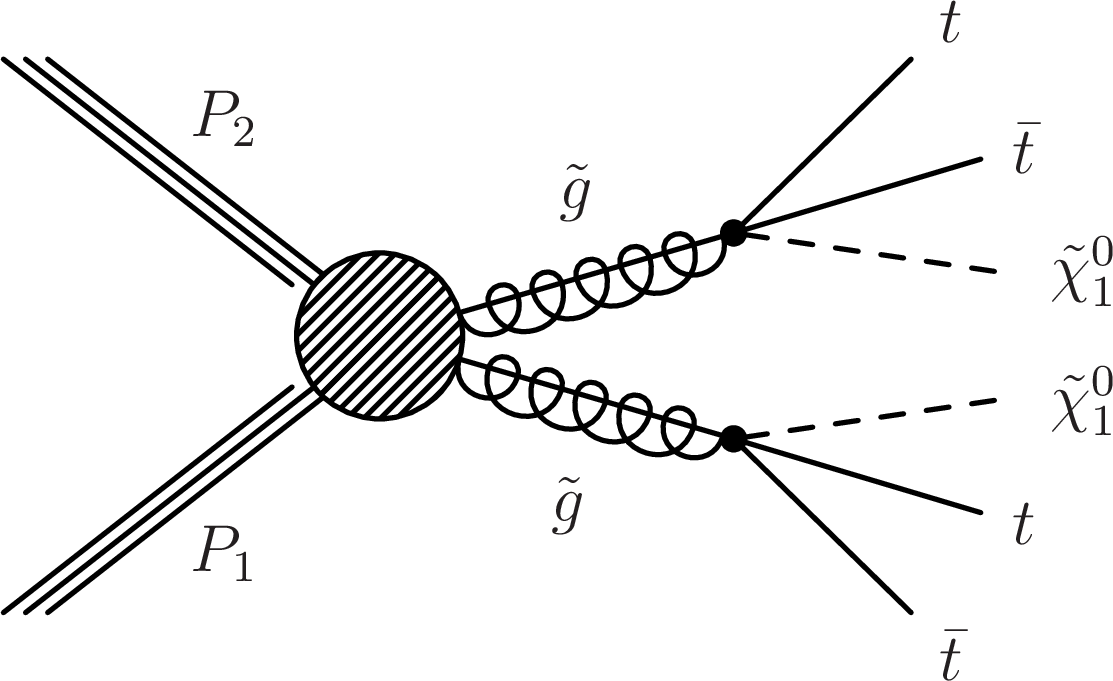
\includegraphics[width=0.3\textwidth]{img/CMS-PAS-SUS-16-014_Figure_001-a.png}
    \caption{The \texttt{T1tttt} model. Versions with bottom and light quarks in the final state were also studied.}
    \label{fig:t1tttt}
\end{figure}
\begin{figure}[]
    \centering
    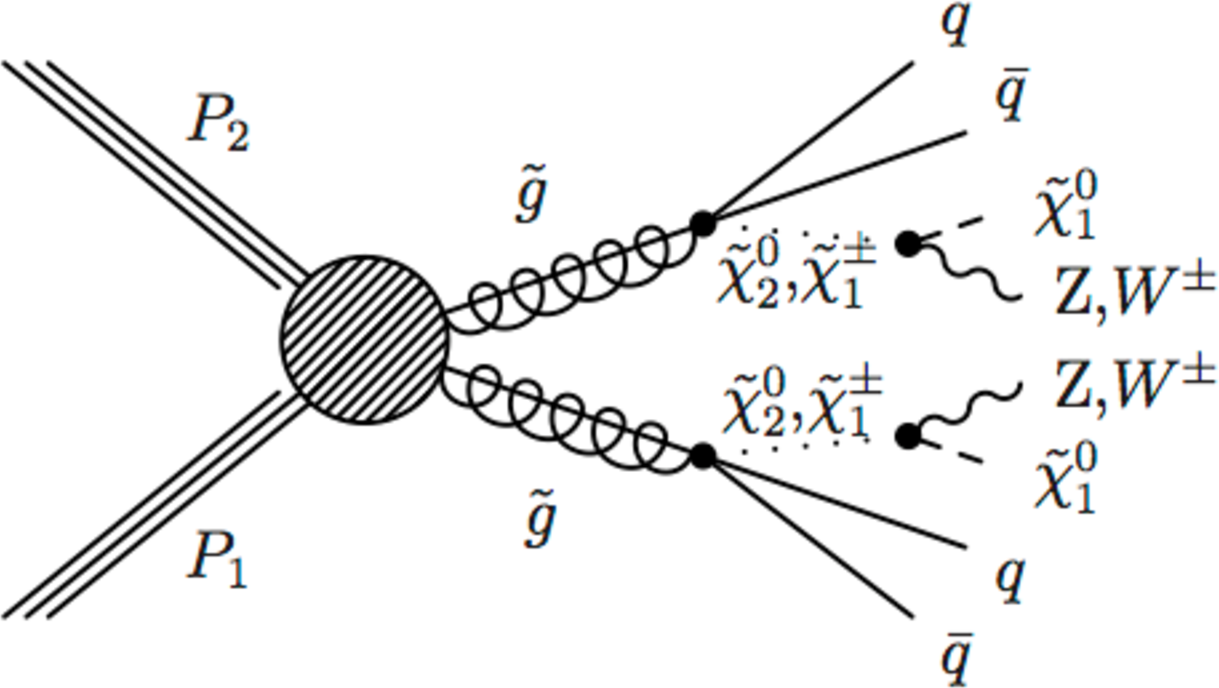
\includegraphics[width=0.3\textwidth]{img/CMS-PAS-SUS-16-014_Figure_001-b.png}
    \caption{The \texttt{T5qqqqVV} model.}
    \label{fig:t5qqqqvv}
\end{figure}
\begin{figure}[]
    \centering
    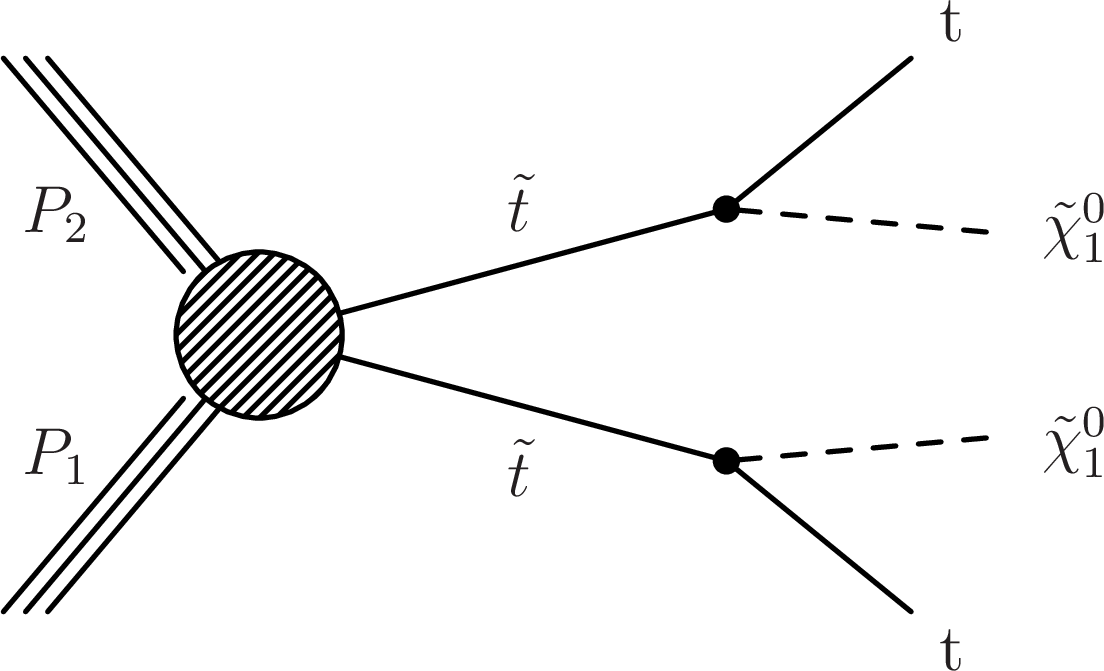
\includegraphics[width=0.3\textwidth]{img/CMS-PAS-SUS-16-014_Figure_001-c.png}
    \caption{The \texttt{T2tt} model.}
    \label{fig:t2tt}
\end{figure}



The search, which originally has more than 172 bins, is also divided into aggregate search regions, as shown together with the search results in \autoref{tab:pre-fit-results-asr}.

\begin{table*}[hp]
  \centering
  \caption{Observed number of events and prefit background predictions
 in the aggregate search regions.}
\label{tab:pre-fit-results-asr}
  \resizebox{\textwidth}{!}{
\begin{tabular}{|c|cccc|cccc||c|c|}
    \hline \hline
 \multirow{2}{*}{Region} &  \multirow{2}{*}{\njets} &  \multirow{2}{*}{\nbjets} &   \multirow{2}{*}{\HT [GeV]} &  \multirow{2}{*}{\MHT [GeV]} & \multirow{2}{*}{ Lost-$e/\mu$} & \multirow{2}{*}{$\tau\rightarrow\mathrm{had}$} & \multirow{2}{*}{$Z\rightarrow\nu\bar{\nu}$} & \multirow{2}{*}{ QCD} & Total & \multirow{2}{*}{ Obs.} \\
 & & &  & & & & & & Pred. & \\
    \hline
1 & 500+ & 500+ & 2+ & 0 & $1056^{+27+59}_{-27-56}$ & $939^{+18+71}_{-18-72}$ & $6530^{+50+380}_{-49-380}$ & $90^{+ 2+35}_{- 2-30}$ & $8615^{+68+400}_{-66-390}$ & 8792 \\ \hline
2 & 750+ & 1500+ & 3+ & 0 & $33.4^{+4.6+2.9}_{-4.5-2.8}$ & $32.3^{+3.2+3.6}_{-3.1-3.6}$ & $374^{+12+46}_{-12-42}$ & $0.62^{+0.06+0.24}_{-0.05-0.22}$ & $441^{+15+46}_{-14-42}$ & 413 \\ \hline
3 & 500+ & 500+ & 5+ & 0 & $212^{+10+15}_{- 9-14}$ & $225^{+ 8+14}_{- 8-15}$ & $763^{+18+47}_{-16-45}$ & $53^{+ 2+20}_{- 2-18}$ & $1254^{+25+55}_{-24-53}$ & 1202 \\ \hline
4 & 750+ & 1500+ & 5+ & 0 & $5.3^{+1.4+0.7}_{-1.2-0.6}$ & $6.3^{+1.2+0.6}_{-0.9-0.6}$ & $55.8^{+4.8+7.6}_{-4.3-6.9}$ & $0.30^{+0.05+0.12}_{-0.05-0.11}$ & $67.7^{+5.5+7.6}_{-4.8-7.0}$ & 79 \\ \hline
5 & 750+ & 1500+ & 9+ & 0 & $0.00^{+0.44+0.00}_{-0.00-0.00}$ & $0.00^{+0.46+0.00}_{-0.00-0.00}$ & $0.00^{+0.64+0.00}_{-0.00-0.00}$ & $0.01^{+0.02+0.00}_{-0.01-0.00}$ & $0.0^{+1.1+0.0}_{-0.0-0.0}$ & 0 \\ \hline
6 & 500+ & 500+ & 2+ & 2+ & $89^{+10+ 6}_{- 8- 5}$ & $91.1^{+5.6+5.4}_{-4.9-5.5}$ & $127^{+ 2+18}_{- 2-18}$ & $15.4^{+0.6+9.6}_{-0.6-8.9}$ & $323^{+16+22}_{-13-21}$ & 350 \\ \hline
7 & 750+ & 750+ & 3+ & 1+ & $59.0^{+7.1+3.9}_{-5.9-3.7}$ & $53.8^{+4.5+3.5}_{-3.9-3.5}$ & $176^{+ 5+16}_{- 4-15}$ & $4.4^{+0.3+1.7}_{-0.3-1.6}$ & $294^{+13+17}_{-11-16}$ & 289 \\ \hline
8 & 500+ & 500+ & 5+ & 3+ & $11.8^{+3.5+0.9}_{-2.7-0.9}$ & $14.9^{+2.5+1.5}_{-2.0-1.5}$ & $11.6^{+0.6+4.9}_{-0.5-4.9}$ & $6.6^{+0.5+7.3}_{-0.5-6.1}$ & $44.8^{+6.1+9.0}_{-4.7-8.0}$ & 34 \\ \hline
9 & 750+ & 1500+ & 5+ & 2+ & $0.9^{+1.5+0.2}_{-0.6-0.2}$ & $1.2^{+1.3+0.2}_{-0.6-0.2}$ & $3.53^{+0.42+0.97}_{-0.29-0.96}$ & $0.15^{+0.09+0.09}_{-0.07-0.08}$ & $5.8^{+2.8+1.0}_{-1.1-1.0}$ & 10 \\ \hline
10 & 750+ & 750+ & 9+ & 3+ & $0.00^{+0.70+0.00}_{-0.00-0.00}$ & $0.53^{+0.72+0.13}_{-0.31-0.13}$ & $0.48^{+0.24+0.33}_{-0.16-0.32}$ & $0.14^{+0.15+0.17}_{-0.13-0.01}$ & $1.2^{+1.4+0.4}_{-0.4-0.3}$ & 3 \\ \hline
11 & 300+ & 300+ & 7+ & 1+ & $329^{+12+21}_{-12-20}$ & $381^{+10+22}_{- 9-22}$ & $194^{+ 8+38}_{- 6-38}$ & $69^{+ 1+29}_{- 1-26}$ & $973^{+23+57}_{-22-55}$ & 896 \\ \hline
12 & 750+ & 750+ & 5+ & 1+ & $37.8^{+5.3+2.7}_{-4.5-2.5}$ & $38.6^{+3.6+2.8}_{-3.1-2.8}$ & $81.7^{+4.1+9.7}_{-3.6-9.6}$ & $3.7^{+0.3+1.5}_{-0.3-1.3}$ & $162^{+10+11}_{- 8-10}$ & 151 \\ \hline
\hline
  \end{tabular}}
\end{table*}




%%%%%%%%%%%%%%%%%%%%%%%%%%%%%%%%%%%%%%%%%%%%%%%%%
The \texttt{Pythia 6.4} settings were read from an external card and are given in \autoref{appendix:pythia}.


In \texttt{MadAnalysis 5}, to run \texttt{DelphesMA5tune} the CMS settings 
with an altered version of this \href{http://madanalysis.irmp.ucl.ac.be/attachment/wiki/PhysicsAnalysisDatabase/delphesMA5tune_card_CMS_SUSY.tcl}{\texttt{DelphesMA5tune} card}, which can be found on the \texttt{MadAnalysis} \href{http://madanalysis.irmp.ucl.ac.be/attachment/wiki/PhysicsAnalysisDatabase/}{Physics Analysis Database} page, were used.
The parameter changed in the \texttt{DelphesMA5tune} card was the b-tag parameter to obtain a b-tag efficiency of 70\%, as shown in \autoref{appendix:delphesma5}.
Cut flows and histograms of several observables are compared with those of CMS in the next sections.
%In the last section, exclusions for the $A$ mass are compared.


\clearpage
%%%%%%%%%%%%%%%%%%%%%%%%%%%%%%%%%%%%%%%%%%%%%%%%%
%%%%%%%%%%%%%%%   Cut flow  %%%%%%%%%%%%%%%%%%%%%%
%%%%%%%%%%%%%%%%%%%%%%%%%%%%%%%%%%%%%%%%%%%%%%%%%

\section{Cut flow}
This analysis is a multijet, missing transverse momentum and zero lepton analysis. The cut flows for the simplified model working points are given in \autoref{tab:sel-eff-gg}, \autoref{tab:sel-eff-qq}, and \autoref{tab:sel-eff-gg-supplementary}.
% The following tables are from Appendix A of the PAS
\begin{table*}[hb]
\caption{
Absolute cumulative efficiencies in \% for each step
of the event selection process
for representative models of gluino pair production.
%(top section) ${m_{\PSg} \gg m_{\PSGczDo}}$
%and (bottom section) ${m_{\PSg} \sim m_{\PSGczDo}}$.
The uncertainties are statistical.
Uncertainties reported as 0.0 correspond to values less than 0.05\%.
}
\small
\begin{center}
\begin{tabular}{l | l | l | l | l |l | l | l}
\hline
\multicolumn{2}{c}{Selection} & \multicolumn{2}{r}{$\Pp\Pp\to\PSg\PSg, \PSg\to\ttbar\PSGczDo$}
     & \multicolumn{2}{r}{$\Pp\Pp\to\PSg\PSg, \PSg\to\bbbar\PSGczDo$}
     & \multicolumn{2}{r}{$\Pp\Pp\to\PSg\PSg, \PSg\to\qqbar\PSGczDo$} \\
\multicolumn{2}{c}{} & \multicolumn{2}{r}{$m_{\PSg}=1500\GeV$} & \multicolumn{2}{r}{$m_{\PSg}=1500\GeV$} & \multicolumn{2}{r}{$m_{\PSg}=1400\GeV$} \\
\multicolumn{2}{c}{} & \multicolumn{2}{r}{$m_{\PSGczDo}=100\GeV$} & \multicolumn{2}{r}{$m_{\PSGczDo}=100\GeV$} & \multicolumn{2}{r}{$m_{\PSGczDo}=100\GeV$} \\
\hline
\njets     & $\geq2$ & \colspacea100.0 & 0.0 & \colspaceb100.0 & 0.0 & \colspacec100.00 & 0.0 \\
\HT        & $>300\GeV$ & \colspacea100.0 & 0.0 & \colspaceb100.0 & 0.0 & \colspacec100.0 & 0.0 \\
\MHT       & $>300\GeV$ & \colspacea76.7 & 0.3 & \colspaceb80.3 & 0.4 & \colspacec80.0 & 0.3 \\
\nmuons    & $=0$ & \colspacea48.6 & 0.4 & \colspaceb79.8 & 0.4 & \colspacec80.0 & 0.3 \\
\nisomuons & $=0$ & \colspacea47.8 & 0.4 & \colspaceb79.6 & 0.4 & \colspacec79.9 & 0.3 \\
\neles     & $=0$ & \colspacea30.7 & 0.3 & \colspaceb79.2 & 0.4 & \colspacec79.5 & 0.3 \\
\nisoeles  & $=0$ & \colspacea29.7 & 0.3 & \colspaceb78.7 & 0.4 & \colspacec79.1 & 0.3 \\
\nisohads  & $=0$ & \colspacea28.3 & 0.3 & \colspaceb78.0 & 0.4 & \colspacec78.3 & 0.3 \\
\dpmht1    & $>0.5$ & \colspacea27.7 & 0.3 & \colspaceb76.7 & 0.4 & \colspacec76.9 & 0.3 \\
\dpmht2    & $>0.5$ & \colspacea25.2 & 0.3 & \colspaceb69.2 & 0.5 & \colspacec69.8 & 0.3 \\
\dpmht3    & $>0.3$ & \colspacea23.7 & 0.3 & \colspaceb63.9 & 0.5 & \colspacec64.4 & 0.3 \\
\dpmht4    & $>0.3$ & \colspacea22.1 & 0.3 & \colspaceb58.6 & 0.5 & \colspacec59.4 & 0.3 \\
\multicolumn{2}{c}{Event quality filter} & \colspacea21.8 & 0.3 & \colspaceb57.7 & 0.5 & \colspacec58.7 & 0.3 \\
\hline
\multicolumn{2}{c}{Selection} & \multicolumn{2}{r}{$\Pp\Pp\to\PSg\PSg, \PSg\to\ttbar\PSGczDo$}
     & \multicolumn{2}{r}{$\Pp\Pp\to\PSg\PSg, \PSg\to\bbbar\PSGczDo$}
     & \multicolumn{2}{r}{$\Pp\Pp\to\PSg\PSg, \PSg\to\qqbar\PSGczDo$} \\
\multicolumn{2}{c}{} & \multicolumn{2}{r}{$m_{\PSg}=1200\GeV$} & \multicolumn{2}{r}{$m_{\PSg}=1000\GeV$} & \multicolumn{2}{r}{$m_{\PSg}=1000\GeV$} \\
\multicolumn{2}{c}{} & \multicolumn{2}{r}{$m_{\PSGczDo}=800\GeV$} & \multicolumn{2}{r}{$m_{\PSGczDo}=900\GeV$} & \multicolumn{2}{r}{$m_{\PSGczDo}=800\GeV$} \\
\hline
\njets     & $\geq2$ & \colspacea100.0 & 0.0 & \colspaceb92.5 & 0.1 & \colspacec99.6 & 0.0 \\
\HT        & $>300\GeV$ & \colspacea99.0 & 0.0 & \colspaceb38.6 & 0.1 & \colspacec81.3 & 0.1 \\
\MHT       & $>300\GeV$ & \colspacea14.9 & 0.1 & \colspaceb14.1 & 01  & \colspacec19.1 & 0.1 \\
\nmuons    & $=0$ & \colspacea9.6 & 0.1 & \colspaceb13.9 & 0.1 & \colspacec19.1 & 0.1 \\
\nisomuons & $=0$ & \colspacea9.2 & 0.1 & \colspaceb13.6 & 0.1 & \colspacec19.1 & 0.1 \\
\neles     & $=0$ & \colspacea6.2 & 0.1 & \colspaceb13.4 & 0.1 & \colspacec19.0 & 0.1 \\
\nisoeles  & $=0$ & \colspacea5.8 & 0.1 & \colspaceb13.1 & 0.1 & \colspacec18.8 & 0.1 \\
\nisohads  & $=0$ & \colspacea5.3 & 0.1 & \colspaceb12.8 & 0.1 & \colspacec18.4 & 0.1 \\
\dpmht1    & $>0.5$ & \colspacea5.3 & 0.1 & \colspaceb12.8 & 0.1 & \colspacec18.4 & 0.1 \\
\dpmht2    & $>0.5$ & \colspacea4.5 & 0.1 & \colspaceb11.4 & 0.1 & \colspacec16.9 & 0.1 \\
\dpmht3    & $>0.3$ & \colspacea4.0 & 0.1 & \colspaceb10.4 & 0.1 & \colspacec15.8 & 0.1 \\
\dpmht4    & $>0.3$ & \colspacea3.6 & 0.1 & \colspaceb9.6 & 0.1 & \colspacec14.8 & 0.1 \\
\multicolumn{2}{c}{Event quality filter} & \colspacea3.5 & 0.1 & \colspaceb9.4 & 0.1 & \colspacec14.6 & 0.1 \\
\hline
\end{tabular}
\label{tab:sel-eff-gg}
\end{center}
\end{table*}

\begin{table*}[htb]
\caption{
Absolute cumulative efficiencies in \% for each step
of the event selection process
for representative models of squark pair production.
%(top section) ${m_{\sQua} \gg m_{\PSGczDo}}$
%and (bottom section) ${m_{\sQua} \sim m_{\PSGczDo}}$.
The uncertainties are statistical.
Uncertainties reported as 0.0 correspond to values less than 0.05\%.
}
\small
\begin{center}
\begin{tabular}{l | l | l | l | l |l | l | l}
\hline
\multicolumn{2}{c}{Selection} & \multicolumn{2}{r}{$\Pp\Pp\to\sTop\PASQt,\sTop\to\cPqt\PSGczDo$}
     & \multicolumn{2}{r}{$\Pp\Pp\to\sBot\PASQb, \sBot\to\cPqb\PSGczDo$}
     & \multicolumn{2}{r}{$\Pp\Pp\to\sQua\PASQ, \sQua\to\cPq\PSGczDo$} \\
\multicolumn{2}{c}{} & \multicolumn{2}{r}{$m_{\sTop}=700\GeV$} & \multicolumn{2}{r}{$m_{\sBot}=650\GeV$} & \multicolumn{2}{r}{$m_{\sQua}=1000\GeV$} \\
\multicolumn{2}{c}{} & \multicolumn{2}{r}{$m_{\PSGczDo}=50\GeV$} & \multicolumn{2}{r}{$m_{\PSGczDo}=1\GeV$} & \multicolumn{2}{r}{$m_{\PSGczDo}=100\GeV$} \\
\hline
\njets     & $\geq2$ & \colspacea99.8 & 0.0 & \colspaceb98.2 & 0.1 & \colspacec98.9 & 0.1 \\
\HT        & $>300\GeV$ & \colspacea96.4 & 0.1 & \colspaceb95.4 & 0.1 & \colspacec98.6 & 0.1 \\
\MHT       & $>300\GeV$ & \colspacea57.8 & 0.3 & \colspaceb59.8 & 0.2 & \colspacec80.0 & 0.3 \\
\nmuons    & $=0$ & \colspacea46.6 & 0.3 & \colspaceb59.6 & 0.2 & \colspacec79.9 & 0.3 \\
\nisomuons & $=0$ & \colspacea46.1 & 0.3 & \colspaceb59.5 & 0.2 & \colspacec79.8 & 0.3 \\
\neles     & $=0$ & \colspacea37.4 & 0.3 & \colspaceb59.2 & 0.2 & \colspacec79.6 & 0.3 \\
\nisoeles  & $=0$ & \colspacea36.9 & 0.3 & \colspaceb59.0 & 0.2 & \colspacec79.3 & 0.3 \\
\nisohads  & $=0$ & \colspacea35.8 & 0.3 & \colspaceb58.5 & 0.2 & \colspacec78.7 & 0.3 \\
\dpmht1    & $>0.5$ & \colspacea35.7 & 0.3 & \colspaceb58.4 & 0.2 & \colspacec78.6 & 0.3 \\
\dpmht2    & $>0.5$ & \colspacea34.0 & 0.3 & \colspaceb55.7 & 0.2 & \colspacec74.5 & 0.3 \\
\dpmht3    & $>0.3$ & \colspacea33.1 & 0.3 & \colspaceb53.3 & 0.2 & \colspacec70.6 & 0.3 \\
\dpmht4    & $>0.3$ & \colspacea31.8 & 0.3 & \colspaceb51.6 & 0.2 & \colspacec67.9 & 0.3 \\
\multicolumn{2}{c}{Event quality filter} & \colspacea31.4 & 0.3 & \colspaceb50.8 & 0.3 & \colspacec67.1 & 0.3 \\
\hline
\multicolumn{2}{c}{Selection} & \multicolumn{2}{r}{$\Pp\Pp\to\sTop\PASQt, \sTop\to\cPqt\PSGczDo$}
     & \multicolumn{2}{r}{$\Pp\Pp\to\sBot\PASQb, \sBot\to\cPqb\PSGczDo$}
     & \multicolumn{2}{r}{$\Pp\Pp\to\sQua\PASQ, \sQua\to\cPq\PSGczDo$} \\
\multicolumn{2}{c}{} & \multicolumn{2}{r}{$m_{\sTop}=300\GeV$} & \multicolumn{2}{r}{$m_{\sBot}=500\GeV$} & \multicolumn{2}{r}{$m_{\sQua}=700\GeV$} \\
\multicolumn{2}{c}{} & \multicolumn{2}{r}{$m_{\PSGczDo}=200\GeV$} & \multicolumn{2}{r}{$m_{\PSGczDo}=300\GeV$} & \multicolumn{2}{r}{$m_{\PSGczDo}=400\GeV$} \\
\hline
\njets     & $\geq2$ & \colspacea86.9 & 0.0 & \colspaceb96.0 & 0.1 & \colspacec98.0 & 0.0 \\
\HT        & $>300\GeV$ & \colspacea23.3 & 0.0 & \colspaceb68.0 & 0.1 & \colspacec91.3 & 0.1 \\
\MHT       & $>300\GeV$ & \colspacea2.84 & 0.0 & \colspaceb15.6 & 0.1 & \colspacec43.8 & 0.1 \\
\nmuons    & $=0$ & \colspacea2.16 & 0.0 & \colspaceb15.6 & 0.1 & \colspacec43.8 & 0.1 \\
\nisomuons & $=0$ & \colspacea2.10 & 0.0 & \colspaceb15.5 & 0.1 & \colspacec43.7 & 0.1 \\
\neles     & $=0$ & \colspacea1.60 & 0.0 & \colspaceb15.4 & 0.1 & \colspacec43.5 & 0.1 \\
\nisoeles  & $=0$ & \colspacea1.52 & 0.0 & \colspaceb15.3 & 0.1 & \colspacec43.4 & 0.1 \\
\nisohads  & $=0$ & \colspacea1.41 & 0.0 & \colspaceb15.2 & 0.1 & \colspacec43.0 & 0.1 \\
\dpmht1    & $>0.5$ & \colspacea1.40 & 0.0 & \colspaceb15.1 & 0.1 & \colspacec42.9 & 0.1 \\
\dpmht2    & $>0.5$ & \colspacea1.03 & 0.0 & \colspaceb14.1 & 0.1 & \colspacec41.1 & 0.1 \\
\dpmht3    & $>0.3$ & \colspacea0.85 & 0.0 & \colspaceb13.5 & 0.1 & \colspacec39.6 & 0.1 \\
\dpmht4    & $>0.3$ & \colspacea0.73 & 0.0 & \colspaceb13.1 & 0.1 & \colspacec38.4 & 0.1 \\
\multicolumn{2}{c}{Event quality filter} & \colspacea0.72 & 0.0 & \colspaceb12.9 & 0.1 & \colspacec37.9 & 0.1 \\
\hline
\end{tabular}
\label{tab:sel-eff-qq}
\end{center}
\end{table*}


\begin{table}[htb]
\caption{Absolute cumulative efficiencies in \% for additional representative models of gluino pair production. The uncertainties are statistical. Uncertainties reported as 0.0 correspond to values less than 0.05\%.}
\small
\begin{center}
\begin{tabular}{l |l | l | l| l | l | l | l | l | l} %MSSSS}
\hline
\multicolumn{2}{c}{Selection} & \multicolumn{2}{r}{$\text{p}\text{p} \to \PSg\PSg, \PSg \to \tbbar \text{W}^{*-} \PSGczDo$} & \multicolumn{2}{r}{$\text{p}\text{p} \to \PSg\PSg, \PSg \to \qqbar \text{V} \PSGczDo$} & \multicolumn{2}{r}{$\text{p}\text{p} \to \PSg\PSg, \PSg \to \tbbar \text{W}^{*-} \PSGczDo$} & \multicolumn{2}{r}{$\text{p}\text{p} \to \PSg\PSg, \PSg \to \qqbar \text{V} \PSGczDo$} \\
\multicolumn{2}{c}{} & \multicolumn{2}{r}{$m_{\PSg}=1500\GeV$} & \multicolumn{2}{r}{$m_{\PSg}=1400\GeV$} & \multicolumn{2}{r}{$m_{\PSg}=1100\GeV$} & \multicolumn{2}{r}{$m_{\PSg}=1000\GeV$} \\
\multicolumn{2}{c}{} & \multicolumn{2}{r}{$m_{\PSGczDo}=100\GeV$} & \multicolumn{2}{r}{$m_{\PSGczDo}=100\GeV$} & \multicolumn{2}{r}{$m_{\PSGczDo}=700\GeV$} & \multicolumn{2}{r}{$m_{\PSGczDo}=800\GeV$} \\
\hline
\njets     & $\geq2$ & \colspace100.0 & 0.0 & \colspace100.0 & 0.0 & \colspace100.0 & 0.0 & \colspace99.7 & 0.0 \\
\HT        & $>300\GeV$ & \colspace100.0 & 0.0 & \colspace100.0 & 0.0 & \colspace98.5 & 0.1 & \colspace70.1 & 0.1 \\
\MHT       & $>300\GeV$ & \colspace77.4 & 0.5 & \colspace73.3 & 0.3 & \colspace31.6 & 0.2 & \colspace13.8 & 0.1 \\
\nmuons    & $=0$ & \colspace56.0 & 0.5 & \colspace61.4 & 0.4 & \colspace25.5 & 0.2 & \colspace11.5 & 0.1 \\
\nisomuons & $=0$ & \colspace53.0 & 0.5 & \colspace61.1 & 0.4 & \colspace24.7 & 0.2 & \colspace11.4 & 0.1 \\
\neles     & $=0$ & \colspace39.7 & 0.5 & \colspace50.0 & 0.4 & \colspace19.9 & 0.2 & \colspace9.6 & 0.1 \\
\nisoeles  & $=0$ & \colspace36.8 & 0.5 & \colspace49.3 & 0.4 & \colspace19.1 & 0.2 & \colspace9.3 & 0.1 \\
\nisohads  & $=0$ & \colspace34.8 & 0.5 & \colspace47.7 & 0.4 & \colspace18.4 & 0.2 & \colspace8.8 & 0.1 \\
\dpmht1    & $>0.5$ & \colspace34.0 & 0.5 & \colspace46.6 & 0.4 & \colspace18.3 & 0.2 & \colspace8.8 & 0.1 \\
\dpmht2    & $>0.5$ & \colspace30.4 & 0.5 & \colspace42.2 & 0.4 & \colspace17.1 & 0.2 & \colspace7.6 & 0.1 \\
\dpmht3    & $>0.3$ & \colspace28.0 & 0.5 & \colspace39.5 & 0.4 & \colspace16.2 & 0.2 & \colspace6.7 & 0.1 \\
\dpmht4    & $>0.3$ & \colspace25.9 & 0.5 & \colspace37.1 & 0.4 & \colspace15.1 & 0.2 & \colspace6.0 & 0.1 \\
\multicolumn{2}{c}{Event quality filter} & \colspace25.7 & 0.5 & \colspace36.6 & 0.4 & \colspace15.0 & 0.2 & \colspace5.9 & 0.1 \\

\label{tab:sel-eff-gg-supplementary}
\end{tabular}
\end{center}
\end{table}


    \clearpage
%%%%%%%%%%%%%%%%%%%%%%%%%%%%%%%%%%%%%%%%%%%%%%%%%
%%%%%%%   Distributions of Observables  %%%%%%%%%
%%%%%%%%%%%%%%%%%%%%%%%%%%%%%%%%%%%%%%%%%%%%%%%%%

\section{Distributions of observables}
In \autoref{fig:fastsim-Nminus1-gg-uncompressed} some kinematic distributions are shown.

\begin{figure}[htb]
  \begin{center}
    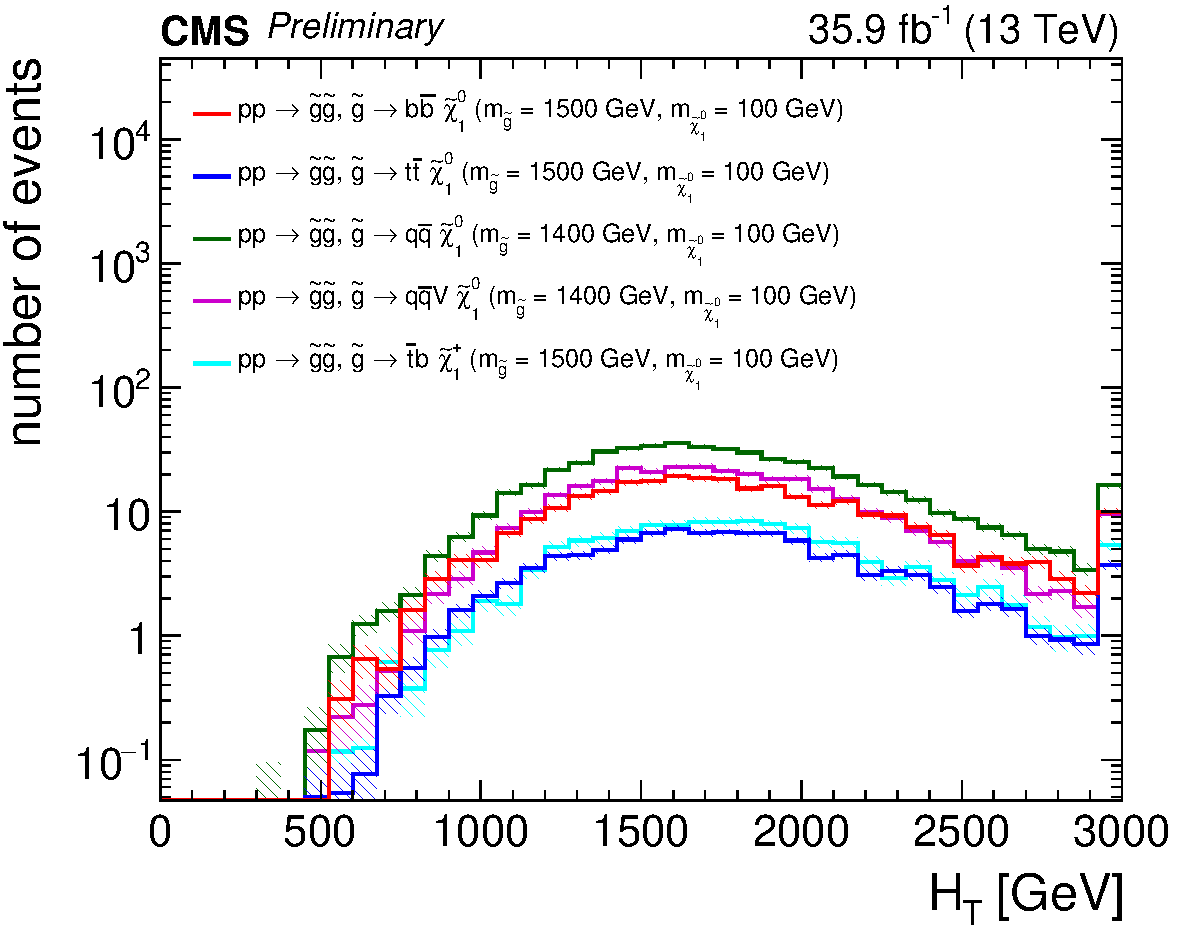
\includegraphics[width=0.48\textwidth]{supplementary/ht_gg_uncompressed_tree_signalMinusHT.pdf}
    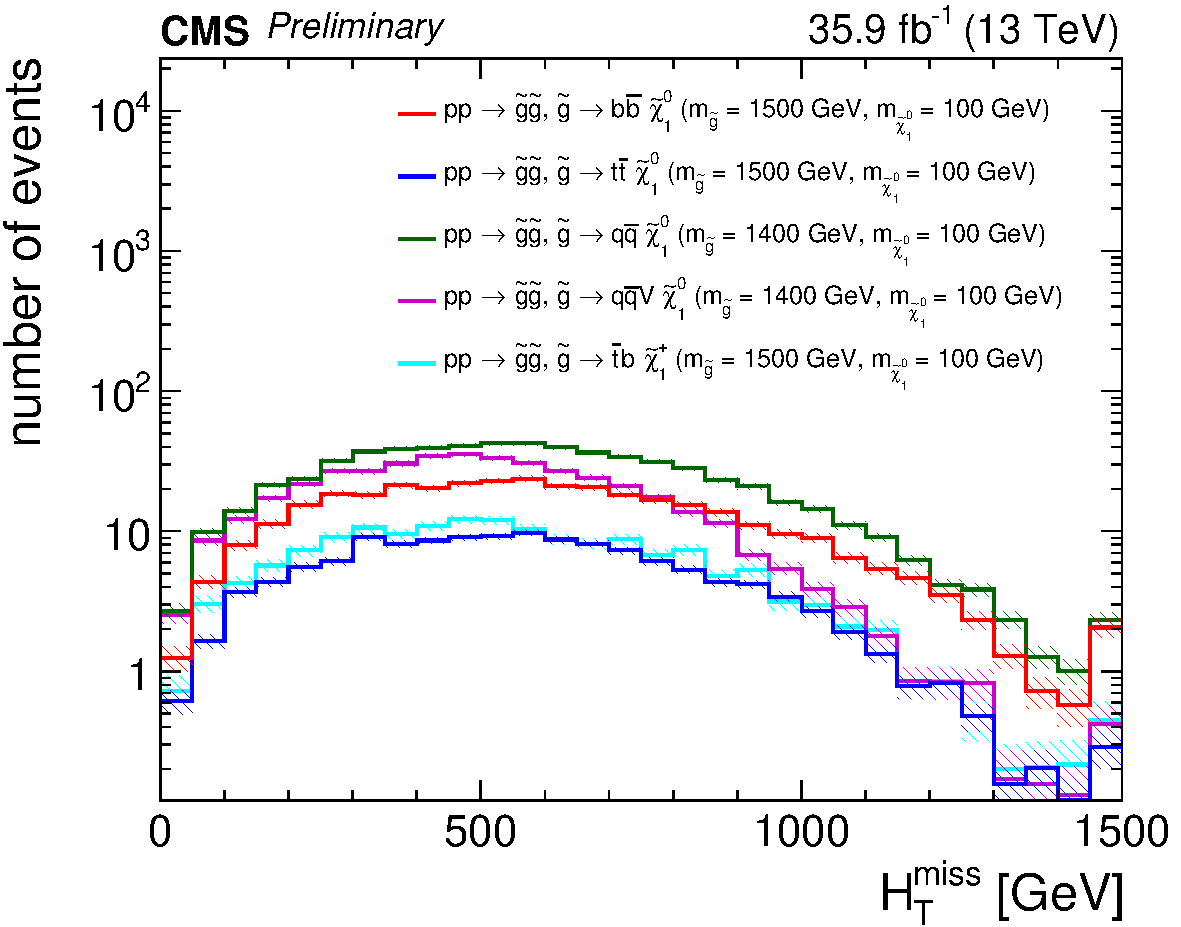
\includegraphics[width=0.48\textwidth]{supplementary/mht_gg_uncompressed_tree_signalMinusMHT.pdf} \\
    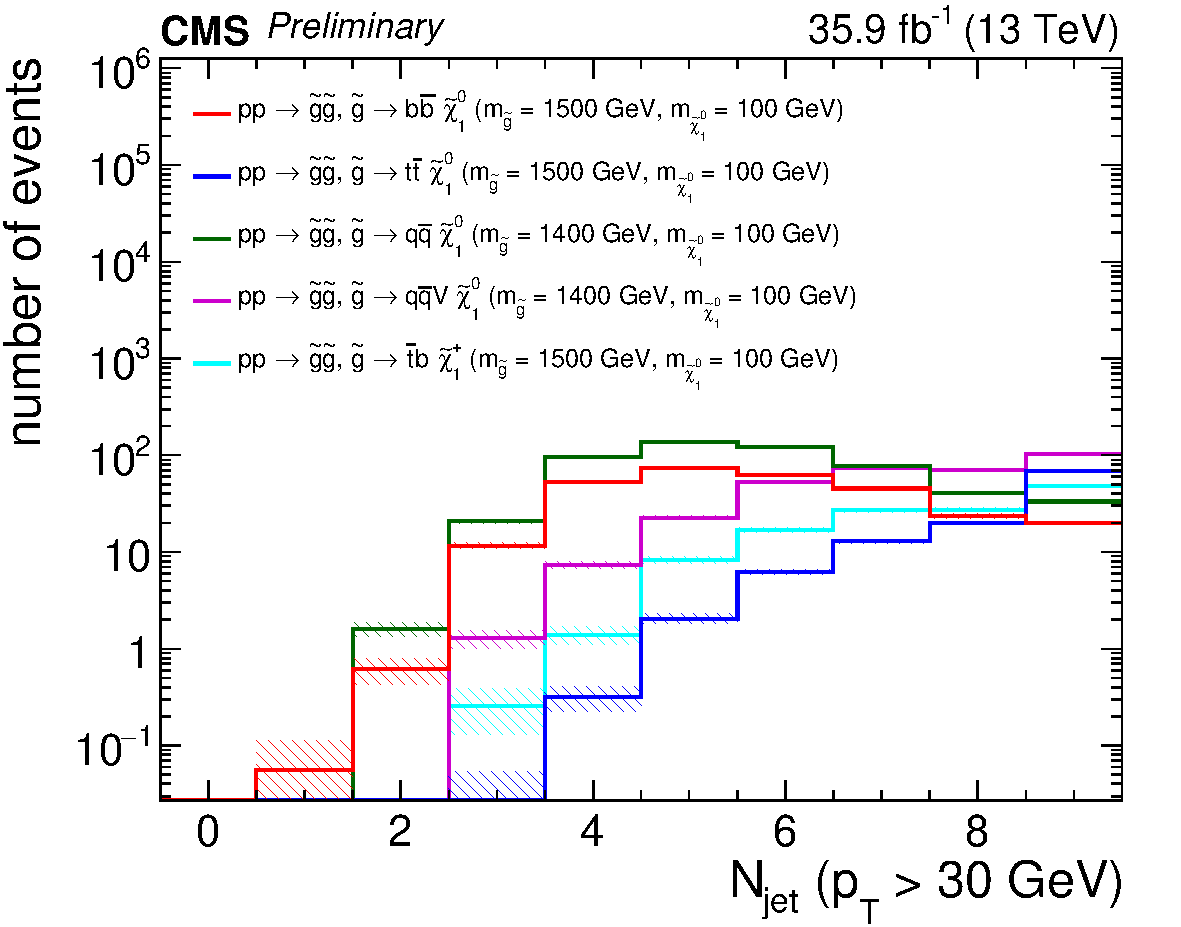
\includegraphics[width=0.48\textwidth]{supplementary/njets_gg_uncompressed_tree_signalMinusNJet.pdf}
    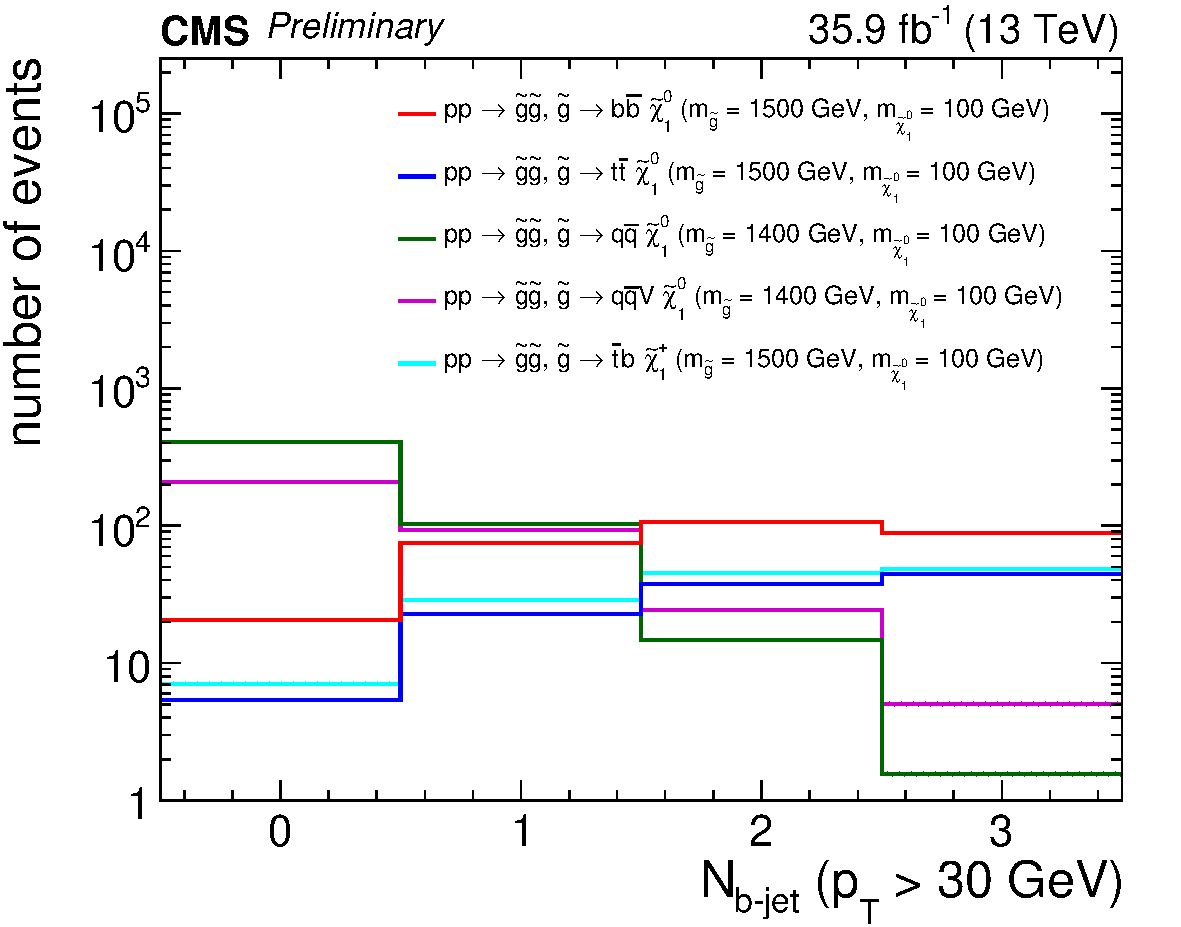
\includegraphics[width=0.48\textwidth]{supplementary/nbjets_gg_uncompressed_tree_signal.pdf}
  \end{center}
  \caption{
    Distributions of (a) $H_{\rm T}$, (b) $H_{\rm T}^{\rm miss}$, (c) the number
    of b-tagged jets, and (d) the number of jets from five representative gluino pair production signal models with ${m_{\PSg} \gg m_{\PSGczDo}}$
    after the baseline selection.
    Each plot ignores the
    baseline requirement (if any) for its respective variable. The
    last bin in each plot contains the overflow events. Only
    statistical uncertainties are shown.\\
  }
  \label{fig:fastsim-Nminus1-gg-uncompressed}
\end{figure}




\clearpage
%%%%%%%%%%%%%%%%%%%%%%%%%%%%%%%%%%%%%%%%%%%%%%%%%
%%%%%%%%%%%%%%% Appendices %%%%%%%%%%%%%%%%%%%%%%
%%%%%%%%%%%%%%%%%%%%%%%%%%%%%%%%%%%%%%%%%%%%%%%%%

\appendix
\appendixpage
\addappheadtotoc

%\clearpage
%%%%%%%%%%%%%%%%%%%%%%%%%%%%%%%%%%%%%%%%%%%%%%%%%
%%%%%%%%%%%%%%% Pythia 6.4 %%%%%%%%%%%%%%%%%%%%%%
%%%%%%%%%%%%%%%%%%%%%%%%%%%%%%%%%%%%%%%%%%%%%%%%%


\section{\texttt{Pythia 6.4} settings}
\label{appendix:pythia}
The following settings in \texttt{Pythia 6.4} as used in \texttt{MadGraph 1.5.12} were read from an external card:
\lstset{language=fortran}
\begin{lstlisting}
!... pythia_card.dat
!...Parton showering on or off
      MSTP(61)=1
      MSTP(71)=1

!...Fragmentation/hadronization on or off
      MSTJ(1)=1

!...Multiple interactions on or off
      MSTP(81)=1

!...Don't stop execution after 10 errors
      MSTU(21)=1

!...Set pdf to cteq6l1:
      MSTP(51)=10042 ! structure function chosen (external PDF CTEQ6L1)
      MSTP(52)=2 ! work with LHAPDF
      LHAPATH=/path/to/lhapdf/PDFSets

!...More settings:
      MSTJ(22)=2 ! Decay those unstable particles
      PARJ(71)=10 . ! for which ctau 10 mm
      MSTP(33)=0 ! no K factors in hard cross sections
      MSTP(2)=1 ! which order running alphaS
      PARP(82)=1.921 ! pt cutoff for multiparton interactions
      PARP(89)=1800. ! sqrts for which PARP82 is set
      PARP(90)=0.227 ! Multiple interactions: rescaling power
      MSTP(96)=6 ! CR (color reconnection parameters)
      PARP(77)=1.016 ! CR
      PARP(78)=0.538 ! CR
      PARP(80)=0.1 ! Prob. colored parton from BBR
      PARP(83)=0.356 ! Multiple interactions: matter distribution parameter
      PARP(84)=0.651 ! Multiple interactions: matter distribution parameter
      PARP(62)=1.025 ! ISR cutoff
      MSTP(91)=1 ! Gaussian primordial kT
      PARP(93)=10.0 ! primordial kT-max
      MSTP(81)=21 ! multiple parton interactions 1 is Pythia default
      MSTP(82)=4 ! Defines the multi-parton model
\end{lstlisting}
In the pythia program \texttt{pythia.f}, the following settings were used:
\begin{lstlisting}
!... pythia.f
C... Model, process
        CALL PYGIVE('MSEL=0')
        CALL PYGIVE('MSUB(186)=1') ! gg->QQbarA (MSSM)
        CALL PYGIVE('KFPR(186,2)= 5') ! Q = b

C... Model params
            IMSS(4)= 2.     ! masses fixed by user',
            RMSS(5)= 30.   ! tan beta',
            RMSS(19)= 30. ! m_A',
            RMSS(1)= 100.  ! M1',
            RMSS(2)= 200.  ! M2',
            RMSS(3)= 800.  ! Mg',
            RMSS(4)= 200.  ! mu',
            RMSS(6)= 1000.  ! MS',
            RMSS(7)= 1000.  ! MS',
            RMSS(8)= 1000.  ! MS',
            RMSS(9)= 1000.  ! MS',
            RMSS(10)= 1000.  ! MS',
            RMSS(11)= 1000.  ! MS',
            RMSS(12)= 1000.  ! MS',
            RMSS(13)= 1000.  ! MS',
            RMSS(14)= 1000.  ! MS',
            RMSS(15)= 2000.  ! Ab',
            RMSS(16)= 2000.  ! At',
            RMSS(17)= 2000.  ! Atau',
            CALL PYGIVE('PMAS(36,1)=30.')  ! mA
C... Switch on decay of A -> mu+mu-:
            CALL PYGIVE('MDME(429,1)=1')  ! decay to mu+mu-',
C... Switch off all other decays:
            CALL PYGIVE('MDME(420,1)=0')  ! Higgs(H) decay into ddbar',
            CALL PYGIVE('MDME(421,1)=0')
            CALL PYGIVE('MDME(422,1)=0')
            CALL PYGIVE('MDME(423,1)=0')
            CALL PYGIVE('MDME(424,1)=0')
            CALL PYGIVE('MDME(425,1)=0')
            CALL PYGIVE('MDME(426,1)=0')
            CALL PYGIVE('MDME(427,1)=0')
            CALL PYGIVE('MDME(428,1)=0')
C... and these as well:
            CALL PYGIVE('MDME(430,1)=0')
            CALL PYGIVE('MDME(431,1)=0')
            ...
            CALL PYGIVE('MDME(502,1)=0')
\end{lstlisting}
The dots indicate the missing incrementing numbers from 432 up to and including 501.

\clearpage
%%%%%%%%%%%%%%%%%%%%%%%%%%%%%%%%%%%%%%%%%%%%%%%%%
%%%%%%%%%%%%  DelphesMA5tune  %%%%%%%%%%%%%%%%%%%
%%%%%%%%%%%%%%%%%%%%%%%%%%%%%%%%%%%%%%%%%%%%%%%%%

\section{\texttt{delphesMA5tune} settings}
\label{appendix:delphesma5}
In \texttt{MadAnalysis 5}, to run \texttt{DelphesMA5tune} the following settings were used:
\lstset{language=sh}
\begin{lstlisting}
ma5>set main.fastsim.package = delphesMA5tune
\end{lstlisting}
and
\begin{lstlisting}
ma5>set main.fastsim.detector = cms
\end{lstlisting}
The \href{http://madanalysis.irmp.ucl.ac.be/attachment/wiki/PhysicsAnalysisDatabase/delphesMA5tune_card_CMS_SUSY.tcl}{\texttt{DelphesMA5tune} card} used for this analysis can be found on the \texttt{MadAnalysis} \href{http://madanalysis.irmp.ucl.ac.be/attachment/wiki/PhysicsAnalysisDatabase/}{Physics Analysis Database} page.
It was adjusted to have an appropriate $b$-tag efficiency:
\lstset{language=sh}
\begin{lstlisting}
###########
# b-tagging
###########

module BTagging BTagging {
  set PartonInputArray Delphes/partons
  set JetInputArray JetEnergyScale/jets

  set BitNumber 0

  set DeltaR 0.5

  set PartonPTMin 1.0

  set PartonEtaMax 2.5

  # default efficiency formula (misidentification rate)
  add EfficiencyFormula {0} {0.01}

  # efficiency formula for c-jets (misidentification rate)
  add EfficiencyFormula {4} {0.20}

  # working point 60%
  # obtained from CMS-SUS-13-013, Section 9
  # efficiency formula for b-jets
  add EfficiencyFormula {5} {
                             (pt < 120.) * ((1.55e-6)*pt^3 + (-4.26e-4)*pt^2 + (0.0391)*pt + (-0.496)) + \
                             (pt >= 120.) * ((-3.26e-4)*pt + 0.7681)
                            }

}
\end{lstlisting}
%  # efficiency formula for b-jets 70%
%  add EfficiencyFormula {5} { 0.70 }



\end{document}
